\documentclass{article}
\usepackage{standalone}
\usepackage{import}
\usepackage{xcolor}

\usepackage{subfigure}

%\usepackage{standalone}
\usepackage{fancyhdr}


\usepackage{import}
\usepackage{caption}
\usepackage{amsfonts, amsmath, amsthm}
\usepackage{makecell}
\usepackage{lastpage}
\usepackage{moresize}



\hyphenpenalty=10000


\usepackage[utf8x]{inputenc}
\usepackage[T1]{fontenc}
\usepackage[english]{babel}
\usepackage{graphicx}
%\usepackage[languagenames,fixlanguage,english]{babelbib}
\usepackage[pdftex]{hyperref}
%\usepackage{txfonts}
%\usepackage{subcaption}
\usepackage[a4paper,top=3cm,bottom=2cm,left=3.5cm,right=3.5cm,marginparwidth=1.75cm]{geometry}
\usepackage{algorithm2e}
\usepackage{pdflscape}

\usepackage[e, gameslogo]{Template/gameshf}






\usepackage{tikz}
\usepackage{pgfplots}
\usepackage{circuitikz}
\usepackage{tabularx}
\usepackage{rotating}
\usepackage{caption} 
\captionsetup[table]{skip=10pt}

\usetikzlibrary{calc,positioning,shapes,decorations.pathreplacing}

\tikzset{
	short/.style={draw,rectangle,text height=3pt,text depth=13pt,
		text width=7pt,align=center,fill=gray!30},
	long/.style={short,text width=1.5cm},
	verylong/.style={short,text width=4.5cm}
}


%% User defined
\newcommand{\N}{\mathbb{N}}
\newcommand{\Z}{\mathbb{Z}}
\newcommand{\Q}{\mathbb{Q}}
\newcommand{\R}{\mathbb{R}}
\newcommand{\C}{\mathbb{C}}
\newcommand{\funcA}{\mathfrak{a}}
\newcommand{\funcB}{\mathfrak{b}}
\newcommand{\funcC}{\mathcal{C}}
\newcommand{\funcU}{\mathcal{U}}
\newcommand{\funcV}{\mathcal{V}}
\newcommand{\funcW}{\mathcal{W}}
\newcommand{\simgrad}{\sym\nabla}
\newcommand{\heps}{{h,\varepsilon}}
\newcommand{\epsh}{{\varepsilon(h)}}
\newcommand{\eps}{{\varepsilon}}
\newcommand{\twoscale}{{\,\overset{2}{\rightharpoonup}\,}}
\newcommand{\drtwoscale}{{\,\overset{dr-2}{\rightharpoonup}\,}}
\DeclareMathOperator{\sym}{sym}
\DeclareMathOperator{\dvg}{div}

\newcommand{\wye}{\mathbin{\tikz[x=1ex,y=1ex]{\draw[line width=.1ex] (0,0)--(30:1)--++(-30:1) (30:1)--++(0,1);}}}
\newcolumntype{Y}{>{\centering\arraybackslash}X}

%\newtheorem{exmp}{Example}[section]
%\newtheorem{note}{Note}
%\newtheorem{theorem}{Theorem}[section]
%\newtheorem{proposition}[theorem]{Proposition}
%\newtheorem{corollary}{Corollary}
%\newtheorem{definition}[theorem]{Definition}
%\newtheorem{lemma}{Lemma}[theorem]

\headheight 40pt              %% put this outside
\headsep 10pt                 %% put this outside


\graphicspath{{./Images/Crane/}{./Images/Electronics/}{./Images/}}

% Source: 
%https://tex.stackexchange.com/questions/117990/unicode-math-breaks-declaremathoperator
\AtBeginDocument{
	\let\div\relax
	\DeclareMathOperator{\div}{div}
}

\usepackage{enumitem}
\setlist[description]{style=unboxed}

%opening
\title{STEM games 2019}
\author{Mentori}

\title{STEM Games Engineering Arena}
\date{}

\begin{document}
	%\maketitle
	
	\thispagestyle{empty}
	\newpage
	\thispagestyle{empty}
	\vspace*{0cm}
	\begin{center}
		
		\textbf{\Huge{STEM Games 2019}}\\
		\vspace*{2.4cm}
		
\includegraphics[width=0.4\textwidth]{logos/engineering} \\
		\vspace*{2.4cm}
		% TODO naslov
		\huge{UNDERWATER HABITATS}
		
		\medskip
		
		\normalsize{a problem by}
		
		\medskip
		
		Dominik Barbarić \\
		Karla Draženović \\
		Nenad Ferdelji \\
		Luka Mandić \\
		Ante Orešković \\
		Ivan Pavić \\
		Vedran Slapničar \\
		Danijel Zadravec \\
		Marko Švec 
		
		\vspace{6cm}
		
		
		% TODO Neki mini tekst?
		\normalsize{}
	\end{center}
	
	\newpage
	
	
\section{Submarine driving}

Finally, the last task of this year's Engineering arena is here! All your calculations in the past 3 days lead you up to this! You have to drive your submarine and transport people and goods to underwater habitats.

A map of the sea bottom is shown in figure \ref{fig:map}. Your task is to visit all 3 habitats and return to the strting position. To visit a habitat you need to be within 3 meters of the habitat for 60 seconds.
Leaving that range resets the timer.

\begin{figure}[!htb]
	\centering
	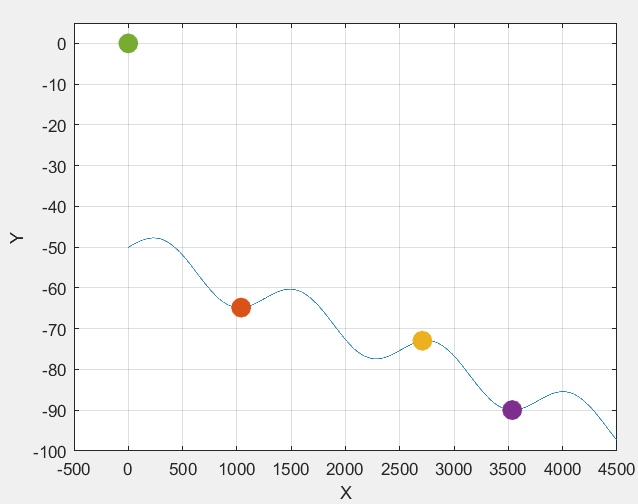
\includegraphics{Images/path.PNG}
	\caption{Map of the sea}
	\label{fig:map}
\end{figure}

Green dot is the start position of the submarine (0, 0). Every other colored dot on map is one habitat you have to visit. Blue line represents bottom of the sea so you have to be careful and not drive your submarine into it. We also provide you with the funtion used to generate the bottom : $0.01*(500*sin(0.005*X)-X) - 50$. Y level zero is the surface of the sea. 

Coliding with the sea bottom is instant fail.

\begin{table}[h!]
	\hyphenpenalty 10000
	\caption{Habitats and coordinates}
	\label{tab:nominalValues}
	\begin{tabularx}{\textwidth}{|Y|Y|Y|} \hline
		\textbf{Habitat} & X[m] & Y[m] \\ \hline 
		\textbf{Red} & 1039   & -64.82\\ \hline 
		\textbf{Yellow} & 2708  & -72.95\\ \hline
		\textbf{Purple} & 3535  &  -89.96\\ \hline
	\end{tabularx}
\end{table}



\begin{figure}[h!]
	\centering
	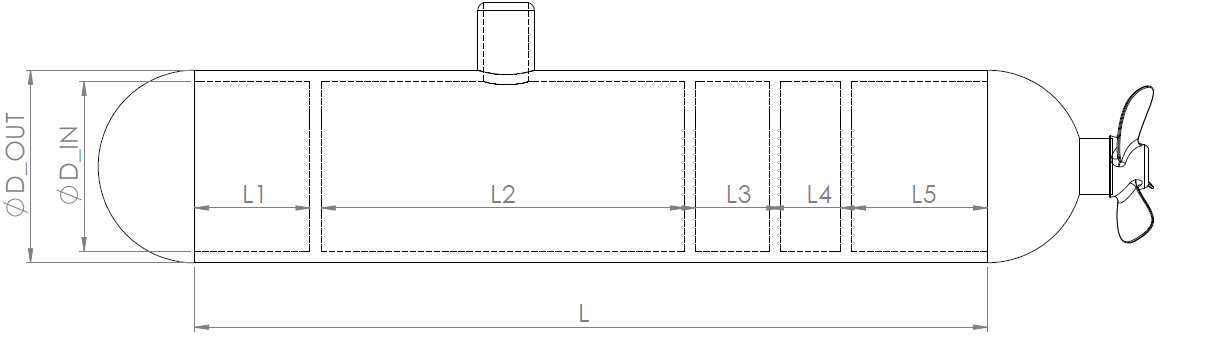
\includegraphics[width=\textwidth]{submarine_side_view.png}
	\caption{Submarine dimensions}
	\label{fig:side_view}
\end{figure}

The following dimensions are given:
\begin{itemize}
	\item $L = 15 \,\textrm{m}$
	\item $D_{OUT} = 3.4 \,\textrm{m}$
	\item $D_{IN} = 3 \,\textrm{m}$
	\item $m = 104.419$ t
	\item $balast\ volume = 30 \ m^3$
	\item $balast\ equilibrium = 50\%$
	\item $ballast\ fill\ speed = 100$ l/s
\end{itemize}


\textbf{Driving references are in this order} : $Red, Yellow, Purple$.


To help you in designing your driving function, GUI will be provided. GUI will allow you to change the submarine inputs and see how the submarine behaves.
 
Based on that, you have to design a regulator as a matlab function with prototype given in your task's folder.

Function output:

\begin{itemize}
	\item[Fuel percentage] - ${0.35,1}$ - Desired \% of fuel pump speed
	\item[Angle] - ${-7,7}$ - In degrees, vector of the output thrust
	\item[Target balast fill] - ${0,1}$ - Desired balast fill \%, the tank fills and empties with the $ballast\ fill\ speed$
	\item[Motor stop] - If this value is 0, the propulsion motor is shut down
	\item[Reverse] - If this value is negative, propulsion motor is reversed
\end{itemize}

Function input:

\begin{itemize}
	\item[pointIndex] - Index of habitat that is current reference point($[1, 2, 3]$ for [$Red, Yellow, Purple$], respectively)
	\item[vx, vy] - X and Y speeds
	\item[sx, sy] - X and Y positions
\end{itemize}


We will grade you \textbf{only by time} to perform whole trip.




\end{document}
